\section{Demostraciones complementarias de SP1}
\label{app:sp1-proofs}

Las afirmaciones formales de la Sección~\ref{subsec:sp1} se demuestran para una decisión lógica estática con costes adimensionales, robots homogéneos y ocupación coherente. Los resultados no se extienden por sí solos a la dinámica Smith muestreada, la comunicación vecinal ni la factibilidad mecánica.

\subsection{Frontera de complejidad}
\label{app:sp1-complexity}

\begin{contribucion}{frontera de complejidad de las cuotas variables}
Con cargas obligatorias y demanda realizable, expandir cada cuota en plazas produce una asignación bipartita con cuotas resoluble en tiempo polinómico. Permitir la selección opcional todo-o-nada bajo presupuesto de robots contiene mochila 0--1 y es NP-difícil.
\end{contribucion}

Si todas las cargas son obligatorias y $\sum_kn_k\leq N$, fije $y_k=1$ en \eqref{eq:sp1-oracle}. Expanda la carga $k$ en $n_k$ plazas indistinguibles y conecte cada robot con cada plaza usando el coste $\kappa_{ik}$. La exclusividad del robot y la ocupación unitaria de cada plaza forman un problema de asignación rectangular o, equivalentemente, una asignación bipartita con cuotas. La matriz de incidencia bipartita es totalmente unimodular. Por ello la relajación lineal tiene un óptimo entero y el problema se resuelve mediante flujo de coste mínimo en tiempo polinómico.

Cuando las cargas son opcionales, tome $\kappa_{ik}=0$ y robots intercambiables. Existe una asignación compatible con un vector $y$ si y solo si $\sum_kn_ky_k\leq N$. El objetivo se reduce a $\max\sum_kv_ky_k$. Identificar $n_k$ con el peso de un objeto, $v_k$ con su valor y $N$ con la capacidad produce exactamente mochila 0--1, que es NP-difícil \parencite{karp1972reducibility}. La transformación es polinómica. Así, la selección todo-o-nada bajo presupuesto es NP-difícil, mientras las cuotas obligatorias aditivas permanecen en la clase polinómica.

\subsection{Potencial y cuotas exactas realizables}
\label{app:sp1-feasible-proof}

Para una desviación unilateral $a_i\to b_i$, el perfil que retira al robot $i$ es el mismo antes y después. Por la utilidad marginal de \eqref{eq:sp1-linear-game},
\[
 U_i(b_i,a_{-i})-U_i(a_i,a_{-i})
 =\Phi_Q(b_i,a_{-i})-\Phi_Q(a_i,a_{-i}).
\]
El juego es, por tanto, de potencial exacto \parencite{monderer1996potential}.

Sea ahora un perfil que no satisface todas las cuotas. Si existe una carga deficitaria y un robot inactivo, incorporarlo reduce $D_n$ en uno y aumenta $C$ a lo sumo en $\kappa_{\max}<\lambda$. La desviación aumenta estrictamente $\Phi_Q$. Si no existe robot inactivo, la identidad
\[
 \sum_kq_k=N\geq\sum_kn_k
\]
implica que un déficit en alguna carga debe coexistir con exceso en otra. Trasladar un robot desde la carga excedida a la deficitaria reduce $D_n+O_n$ en dos. La variación del coste pertenece a $[-\kappa_{\max},\kappa_{\max}]$ y la mejora vuelve a ser estricta. Si existe exceso sin déficit, retirar un robot redundante reduce $O_n$ y no aumenta $C$. Ningún perfil inexacto es Nash.

Recíprocamente, en un perfil con $q_k=n_k$ para toda carga, un robot asignado que pasa a inactividad crea una unidad de déficit y ahorra como máximo $\kappa_{\max}$. Trasladarlo a otra carga crea una unidad de déficit y una de exceso, mientras que la entrada de un robot inactivo crea exceso. Como $\lambda>\kappa_{\max}$, ninguna desviación es rentable. Los Nash puros coinciden exactamente con los perfiles de cuotas correctas.

Cada mejora estricta aumenta $\Phi_Q$ y el espacio contiene $(K+1)^N$ perfiles, de modo que toda trayectoria de mejora termina. Finalmente, desde cualquier perfil inexacto existe una mejora, por lo cual ningún máximo global puede ser inexacto. Sobre el conjunto exacto se cumple $D_n=O_n=0$ y maximizar $\Phi_Q=-C$ equivale a minimizar el coste espacial. Esto completa la Proposición~\ref{thm:sp1-feasible-nash}.

\paragraph{Corolario de regulación estratégica realizable.}
Con cargas obligatorias, $z_{1,k}=q_k-n_k$. Mientras $\boldsymbol z_1\neq\boldsymbol0$, el perfil no satisface todas las cuotas y, por la proposición anterior, no es Nash. Por tanto, existe una mejora estricta. Bajo una activación que no omite indefinidamente a robots con mejora, cada evento aceptado aumenta $\Phi_Q$ y el espacio finito impide una sucesión infinita. La trayectoria alcanza así $\boldsymbol z_1=\boldsymbol0$ en un número finito de revisiones, lo que demuestra el Corolario~\ref{cor:sp1-strategic-regulation}. El argumento se refiere al juego finito de mejora estricta y no prueba convergencia de Smith muestreado ni del cierre QR bajo escasez.

\subsection{Escasez e incentivo de cuórum}
\label{app:sp1-scarcity-proof}

Bajo los supuestos de la Proposición~\ref{thm:sp1-scarcity-degeneracy}, $q_k\leq n_k$ anula todos los términos de exceso y todos los robots activos satisfacen $\sum_kq_k=N$. Por consiguiente,
\[
 D_n(a)=\sum_k(n_k-q_k)=\sum_kn_k-N,
\]
que no depende de la distribución. El coste espacial todavía puede ordenar perfiles, pero el déficit lineal no contiene información sobre cuántas cargas quedan completas.

Para $\beta>0$ y $0\leq q<n_k$, el incremento discreto del beneficio de \eqref{eq:sp1-quorum-benefit} es
\[
 \Delta B_{\beta,k}(q+1)
 =\frac{\exp(\beta q/n_k)\{\exp(\beta/n_k)-1\}}{\exp(\beta)-1}.
\]
Todos los factores salvo $\exp(\beta q/n_k)$ son positivos y constantes respecto de $q$. Los incrementos son, por tanto, estrictamente crecientes antes del cuórum. La saturación mediante $\min\{q,n_k\}$ hace nulo todo incremento posterior.

En el caso $n_1=n_2=N=2$, valores unitarios y costes nulos, la concentración $(2, 0)$ produce beneficio uno. La dispersión $(1, 1)$ produce
\[
 2B_{\beta,k}(1)
 =2\frac{\exp(\beta/2)-1}{\exp(\beta)-1}
 =\frac{2}{\exp(\beta/2)+1}<1
\]
para todo $\beta>0$. El incentivo rompe la indiferencia del déficit lineal en este caso mínimo. Esta desigualdad no afirma que todo máximo local o toda trayectoria Smith seleccione globalmente el mejor subconjunto de cargas.

\clearpage
\subsection{Mapa complementario de sensibilidad}
\label{app:sp1-beta-map}

La Figura~\ref{fig:sp1-beta-map} conserva el barrido de desarrollo sin ocupar el cuerpo principal. El mapa describe el valor obtenido después del cierre y no prueba estabilidad de la dinámica continua ni optimalidad del parámetro.
\begin{figure}[H]
 \centering
 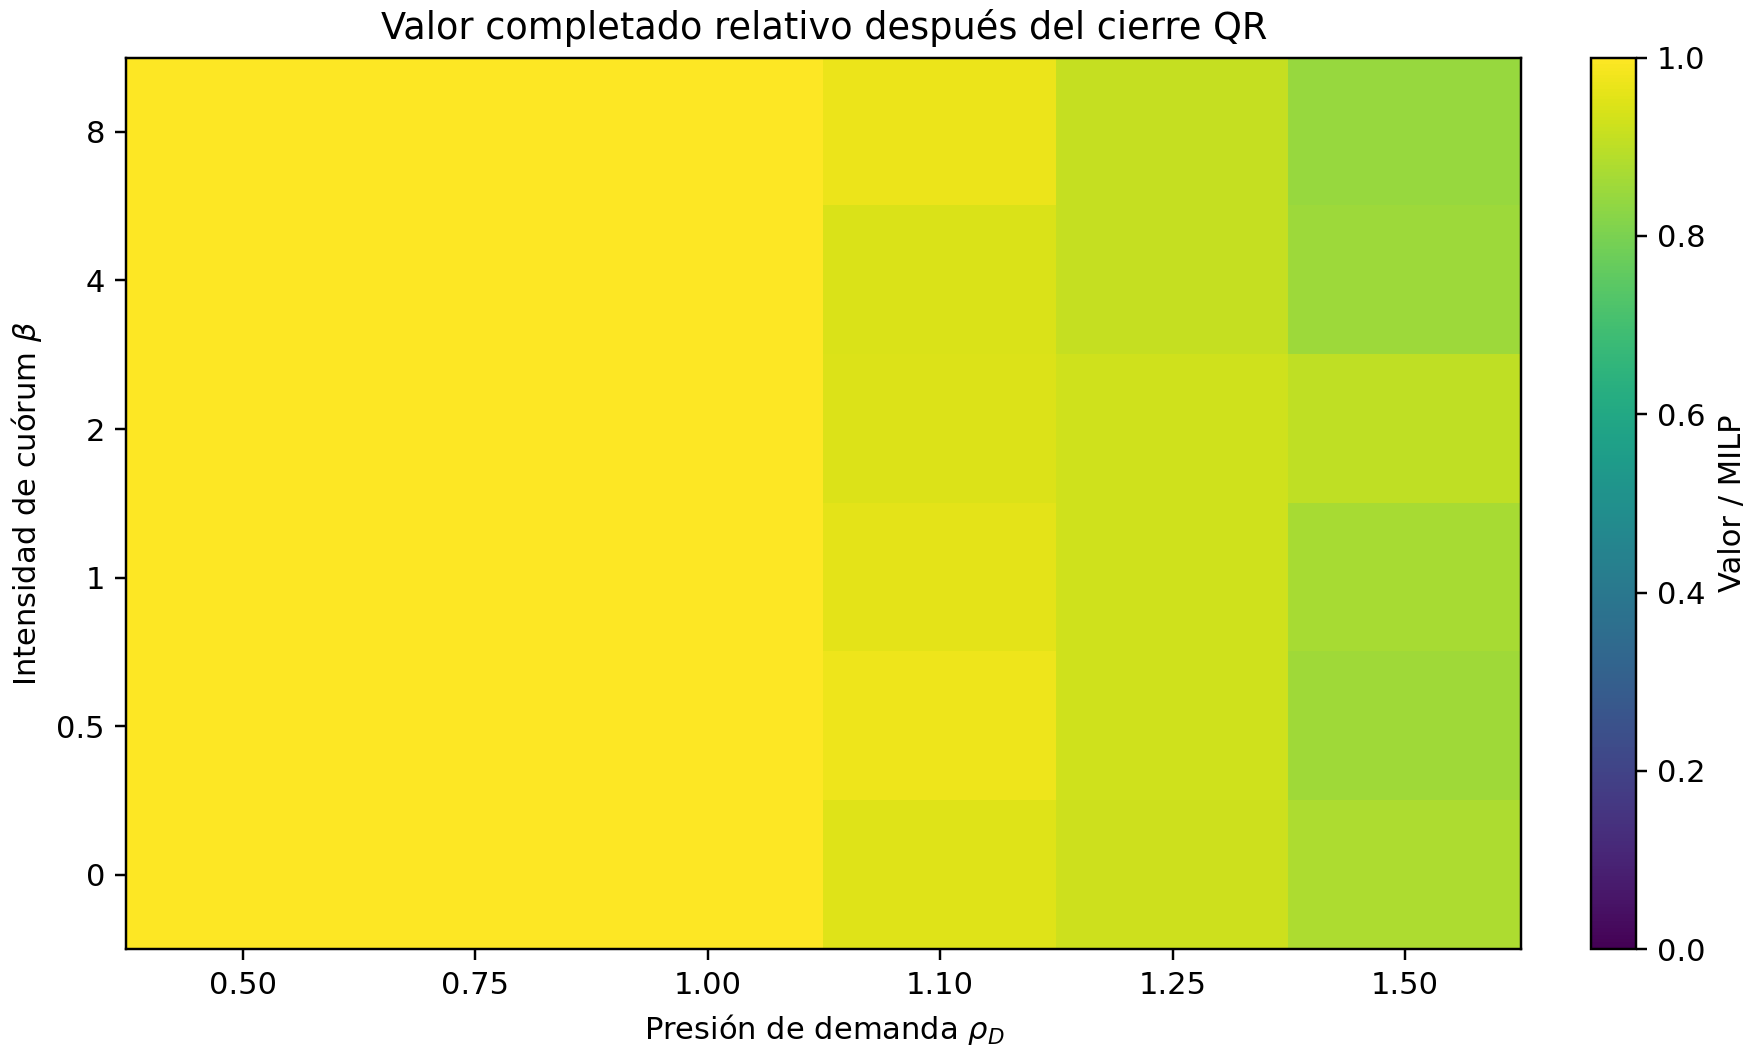
\includegraphics[width=0.76\textwidth]{../results/sp1/SP1_QUORUM_v1/figures/fig-sp1-beta-regime-map.pdf}
 \caption{Mapa de desarrollo $(\rho_D,\beta)$ del valor completado por Smith-QR respecto al MILP. Cada celda promedia diez mundos mixtos con $N=16$.}
 \label{fig:sp1-beta-map}
 \viuownsource
\end{figure}
